\documentclass{article}
\usepackage{graphicx}
\graphicspath{{./figs/}}{}
\usepackage{listings}
\title{
RTL-Assignment 1
}
\begin{document}
\maketitle
\hfill \textbf{Sampath Govardhan} \\
\null \hfill \textbf{FWC22071}\\
\tableofcontents
\section{Module Code}
\begin{lstlisting}
`timescale 1ns / 1ps
//////////////////////////////////////////////////////////////////////////////////
// Company: 
// Engineer: 
// 
// Create Date: 11/23/2022 12:31:22 PM
// Design Name: 
// Module Name: counter
// Project Name: 
// Target Devices: 
// Tool Versions: 
// Description: 
// 
// Dependencies: 
// 
// Revision:
// Revision 0.01 - File Created
// Additional Comments:
// 
//////////////////////////////////////////////////////////////////////////////////


module counter(
    input [7:0] in,
    input clk,
    input latch,
    input div,
    input dec,
    output reg [7:0]count,
    output reg zero
    );

    always @(posedge clk)
    begin
    case({latch,dec})
    2'b10: begin
    count<=in;
    end
    2'b01: begin
    if (count==8'b00000000) begin
    zero =1;
    end
    else begin
    count<=count-1;
    end
    end
    2'b11: begin
    count<=in;
    if (count == 8'b00000000) begin
    zero = 1; 
    end
    else begin
    count<=count-1;
    end
    end
    2'b00: begin
    if(div) begin
    count = count/2;
    end 
    end
    endcase
    end
endmodule


\end{lstlisting}



\section{Test Bench Code}
\begin{lstlisting}
`timescale 1ns / 1ps
//////////////////////////////////////////////////////////////////////////////////
// Company: 
// Engineer: 
// 
// Create Date: 11/23/2022 02:21:29 PM
// Design Name: 
// Module Name: counter_tb
// Project Name: 
// Target Devices: 
// Tool Versions: 
// Description: 
// 
// Dependencies: 
// 
// Revision:
// Revision 0.01 - File Created
// Additional Comments:
// 
//////////////////////////////////////////////////////////////////////////////////


module counter_tb();
reg CLK,LATCH,DIV,DEC;
reg [7:0] IN;
wire [7:0] COUNT;
wire ZERO;

counter dut(.in(IN),.clk(CLK),.latch(LATCH),.div(DIV),.dec(DEC),.count(COUNT),.zero(ZERO));
initial begin
CLK = 0;
forever #5 CLK = ~CLK;
end
initial begin
IN=8'b00010000;LATCH=1;DEC=0;
#10
IN=8'd0;LATCH=0;DEC=0;DIV=1;
#10
IN=8'b00000010;LATCH=0;DEC=0;DIV=1;
#10
IN=8'd11;LATCH=0;DEC=0;DIV=1;
#10
LATCH=0;DEC=1;DIV=0;
#10
IN=1;LATCH=0;DEC=1;DIV=0;
#10
LATCH=0;DEC=1;DIV=0;
#10
$stop;
end
endmodule

\end{lstlisting}
\section{Timing diagram}
\begin{figure}[h]
    \centering
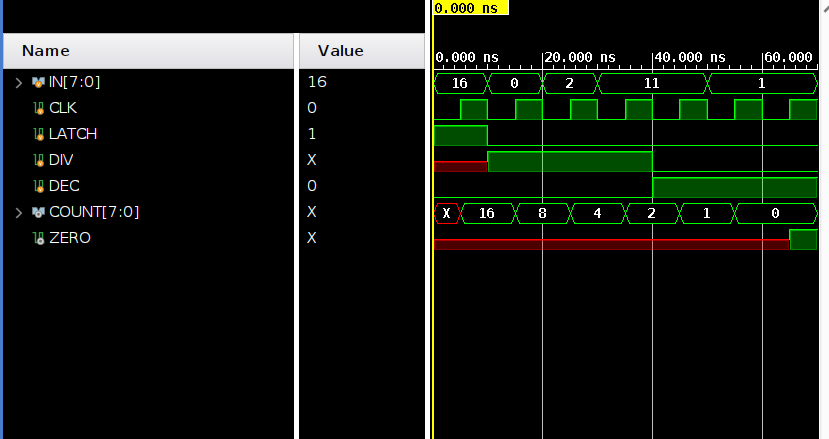
\includegraphics[width=\columnwidth]{figs/timing diagram.png}
    \caption{Timing diagram}
    \label{fig:my_label}
\end{figure}
\vspace{10cm}

\section{Schematic diagram}
\begin{figure}[h]
    \centering
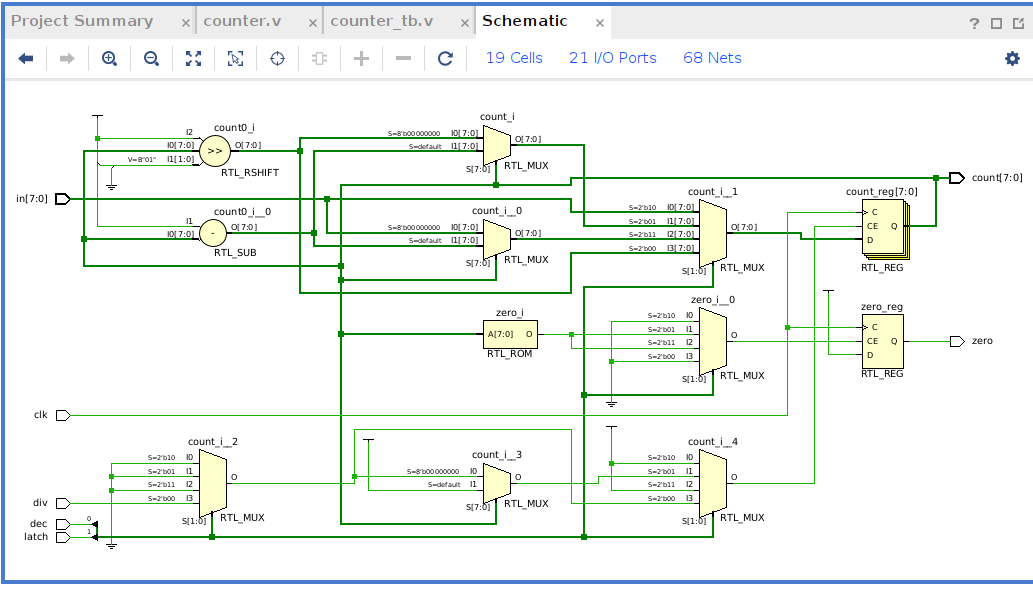
\includegraphics[width=\columnwidth]{figs/schematic diagram.png}
    \caption{Netlist}
    \label{fig:my_label}
\end{figure}
\vspace{10cm}

\section{Design diagram}
\begin{figure}[h]
    \centering
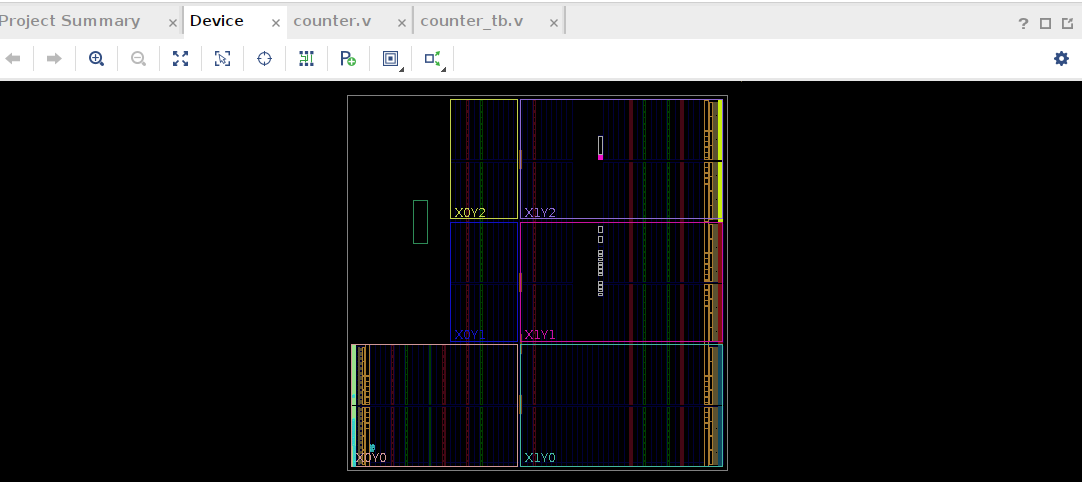
\includegraphics[width=\columnwidth]{figs/design diagram.png}
    \caption{Design diagram}
    \label{fig:my_label}
\end{figure}
\end{document}
